\section{The ranked probability score (RPS)}
\label{app:rps}
% Provenance: every worked-example number is printed by paper_latex_and_notes/AAAI_2027_EvalAIScientists_JudgesKL/rps_appendix_examples.py;
% make_memo_assets.py runs that script and logs its output in assets_log.txt. The archived-experiment-11 numbers come from
% experiments/archive/11_formulation4_train_only_ce_mixture_cv_start_10Nov2026_end_10Nov2026/results.md.

This appendix defines the ranked probability score (RPS), gives three ways to read it, proves that it is strictly proper, shows what it detects that mean-based metrics cannot, and states its limits.
RPS is not a standard machine-learning metric, so we write out every step.
A script prints every number below (\texttt{rps\_appendix\_examples.py}); the identities in this appendix hold to $2.2\times10^{-15}$ or better on random forecasts.

\subsection{Definition}
\label{app:rps-def}

A human rating is an ordered category $r\in\{0,1,\dots,5\}$.
For an item, a judge outputs a forecast $q=(q_0,\dots,q_5)$.
Its cumulative distribution function (CDF) and survival function are
\begin{equation}
Q_j=\Pr_q[R\le j]=\sum_{k=0}^{j}q_k,\qquad S_j=\Pr_q[R>j]=1-Q_j,\qquad j=0,\dots,4 .
\end{equation}
We omit the threshold $j=5$ because $Q_5=1$ for every forecast.
The ranked probability score~\citep{epstein1969scoring} compares the judge's CDF with the step function of the observed rating:
\begin{align}
L_{\RPS}(q,r)&=\frac15\sum_{j=0}^{4}\bigl(Q_j-\Ind\{r\le j\}\bigr)^2 \label{eq:rps-cdf}\\
&=\frac15\sum_{j=0}^{4}\bigl(S_j-\Ind\{r>j\}\bigr)^2 .\label{eq:rps-sf}
\end{align}
We use it as a loss: lower is better.
Dividing by the five thresholds puts it in $[0,1]$.
It equals 0 when $q$ puts all its mass on $r$, and it equals 1 when $q$ puts all its mass on the opposite end of the scale (a point mass on rating 0 scored against a rating of 5).
Some references omit the factor $1/5$, and their values are five times ours.

For $N$ items $x_i$ with $n_i$ human ratings $r_{i1},\dots,r_{in_i}$ each, we average over the ratings of an item and then over items:
\begin{equation}
\widehat{\RPS}=\frac1N\sum_{i=1}^{N}\frac1{n_i}\sum_{m=1}^{n_i}L_{\RPS}(q_i,r_{im}).
\end{equation}
Writing $\hat P_{ij}$ for the empirical CDF of item $i$'s ratings, the inner average equals $\frac15\sum_j\bigl[(Q_{ij}-\hat P_{ij})^2+\hat P_{ij}(1-\hat P_{ij})\bigr]$.
A single rating per item already gives an unbiased estimate of the judge's expected score, so we estimate no per-item histogram.

\subsection{Three ways to read RPS}
\label{app:rps-read}

\paragraph{Five yes/no questions.}
At each threshold $j$ the judge answers ``is the rating at most $j$?'' with probability $Q_j$, and the human rating supplies the answer.
Each summand in \Cref{eq:rps-cdf} is the Brier score of one such binary forecast, so RPS is the average Brier score over the five threshold questions.
Equation~\ref{eq:rps-sf} says the same for the chance that the rating exceeds each threshold.

\paragraph{Distance between staircases.}
The judge's CDF is a staircase that rises from 0 to 1, and the observed rating is a single step at $r$.
RPS sums the squared vertical gaps between the two staircases, so a near miss leaves gaps at few thresholds and a far miss at many.
\Cref{fig:rps-staircase} works one example: for the forecast $q=(0,0,0.1,0.3,0.4,0.2)$ and the rating $r=4$, the cumulative probabilities are $Q=(0,0,0.1,0.4,0.8)$, the squared gaps are $(0,0,0.01,0.16,0.04)$ and RPS is $0.21/5=0.042$.
\Cref{tab:rps-examples} compares four forecasts against the same rating.
Cross-entropy (CE) is infinite for every forecast with $q_4=0$, and the categorical Brier score $\sum_k(q_k-\Ind\{r=k\})^2$ equals 2 for every point mass away from 4.
Only RPS scores the near miss (all mass on rating 5, RPS 0.200) better than the far miss (all mass on rating 0, RPS 0.800).
A point mass $d$ ratings away from the observed rating scores $d/5$: 0.0, 0.2, 0.4, 0.6 and 0.8 for $d=0,\dots,4$.

\begin{figure}[t]
\centering
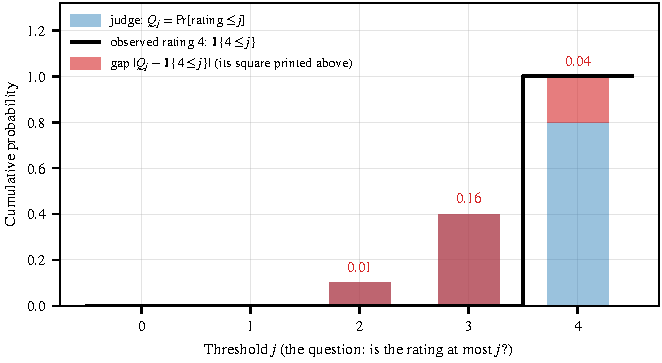
\includegraphics[width=0.62\textwidth]{figures/fig_rps_staircase.pdf}
\caption{\textbf{RPS adds the squared gaps between the judge's cumulative probabilities and the observed rating's step.}
Constructed example, not data: the judge's forecast over ratings 0 to 5 is $(0,0,0.1,0.3,0.4,0.2)$ and the human rating is 4.
Horizontal axis: the five thresholds $j$; vertical axis: cumulative probability.
Blue bars: the judge's $Q_j=\Pr[\text{rating}\le j]$; black staircase: the observed rating's step $\Ind\{4\le j\}$; red: the gap, with its square printed above.
RPS $=(0.01+0.16+0.04)/5=0.042$ (range 0 to 1, lower is better; a perfect forecast scores 0).}
\label{fig:rps-staircase}
\end{figure}

\begin{table}[t]
\caption{\textbf{Only RPS scores a near miss better than a far miss.}
Scores of four forecasts against one human rating $r=4$ (lower is better for all three scores).
RPS: ranked probability score, range 0 to 1.
Brier: categorical Brier score $\sum_k(q_k-\Ind\{r=k\})^2$, range 0 to 2.
CE: cross-entropy $-\log q_4$ in nats, infinite when $q_4=0$.}
\label{tab:rps-examples}
\centering\small
\begin{tabular}{lccc}
\toprule
Forecast for $r=4$ & RPS & Brier & CE \\
\midrule
all mass on 4 & 0.000 & 0.0 & 0 \\
all mass on 5 & 0.200 & 2.0 & $\infty$ \\
all mass on 0 & 0.800 & 2.0 & $\infty$ \\
half on 3, half on 5 & 0.100 & 1.5 & $\infty$ \\
\bottomrule
\end{tabular}
\end{table}

\paragraph{Rating points.}
For integer ratings, RPS has an absolute-error form, the discrete case of the identity for the continuous ranked probability score~\citep{matheson1976scoring,gneiting2007strictly}:
\begin{equation}
5\,L_{\RPS}(q,r)=\E_q|R-r|-\tfrac12\E_q|R-R'| ,
\label{eq:rps-abs}
\end{equation}
where $R$ and $R'$ are independent draws from $q$.
The first term is the expected distance, in rating points, between a rating sampled from the judge and the human rating.
The second term subtracts half of the judge's own spread, so the score does not penalize a judge merely for spreading its probability.
To see \Cref{eq:rps-abs}, write $|a-r|=\sum_{j=0}^{4}\bigl|\Ind\{a\le j\}-\Ind\{r\le j\}\bigr|$ for integers $a$ and $r$; taking the expectation over $a\sim q$ gives $\E_q|R-r|=\sum_j[Q_j+o_j(1-2Q_j)]$ with $o_j=\Ind\{r\le j\}$, and $\E_q|R-R'|=2\sum_jQ_j(1-Q_j)$, so the right-hand side of \Cref{eq:rps-abs} equals $\sum_j(Q_j-o_j)^2$ because $o_j^2=o_j$.

\subsection{RPS is strictly proper}
\label{app:rps-proper}

Let the human rating be drawn from $p$ with CDF $P$.
Then, for each threshold, $\E[(Q_j-\Ind\{R\le j\})^2]=Q_j^2-2Q_jP_j+P_j=(Q_j-P_j)^2+P_j(1-P_j)$, and summing over the thresholds gives
\begin{equation}
\E_{R\sim p}\bigl[L_{\RPS}(q,R)\bigr]=\underbrace{\frac15\sum_{j=0}^{4}(Q_j-P_j)^2}_{\text{excess: the judge's error}}+\underbrace{\frac15\sum_{j=0}^{4}P_j(1-P_j)}_{\text{rater disagreement}} .
\label{eq:rps-decomposition}
\end{equation}
The second term does not depend on $q$: it is the irreducible disagreement among raters.
The first term is nonnegative, and it vanishes only when $Q_j=P_j$ at every threshold, that is, when $q=p$.
So RPS is strictly proper~\citep{gneiting2007strictly}: a judge minimizes its expected RPS only by reporting the full human rating distribution, including how much the raters disagree.
The script checks \Cref{eq:rps-abs,eq:rps-decomposition} on 2{,}000 random forecasts and distributions, with a maximum absolute error of $1.8\times10^{-15}$.

\subsection{What mean-based metrics miss}
\label{app:rps-mean}

\paragraph{An example of disagreement that correlation cannot see.}
Suppose raters split evenly between ratings 3 and 5 on an item.
Judge~A forecasts the human distribution, and judge~B puts all its mass on rating 4.
Both have expected rating 4.0, so replacing one forecast by the other cannot change a correlation computed from expected ratings across a panel of items; if all expected ratings are constant, the correlation is undefined for both judges.
Judge~A has expected RPS 0.10, which is all irreducible disagreement, whereas judge~B has 0.20.
A uniform forecast over ratings 0 to 5 scores 0.206.

\paragraph{The mean is the sum of the survival function.}
For ratings in $\{0,\dots,5\}$,
\begin{equation}
\E_q[R]=\sum_{j=0}^{4}\Pr_q[R>j]=\sum_{j=0}^{4}S_j .
\label{eq:mean-survival}
\end{equation}
Mean squared error between expected ratings depends on a forecast only through this sum, and correlation across items is weaker still, because shifting or positively rescaling the sums leaves it unchanged.
Survival gaps of opposite sign at different thresholds therefore cancel in every mean-based metric.
RPS squares the gap at each threshold before adding, so the gaps cannot cancel.
In the example, judge~A has $S=(1,1,1,0.5,0.5)$ and judge~B has $S=(1,1,1,1,0)$.
Both sum to 4, so their gaps $(0,0,0,+0.5,-0.5)$ cancel in the mean, while their squares give the excess expected RPS $(0.25+0.25)/5=0.10$.
The script checks \Cref{eq:mean-survival} on 1{,}000 random forecasts, with a maximum absolute error of $2.2\times10^{-15}$.

\subsection{Why the cumulative form: scoring with a few ratings per item}
\label{app:rps-sparse}

Each item has two or three human ratings in our retrospective studies, so its empirical histogram leaves at least three of the six bins empty.
For a forecast that gives positive mass to an unobserved rating, the Kullback--Leibler (KL) divergence $\KL(q\|\hat p)$ from the empirical histogram $\hat p$ is infinite unless we smooth $\hat p$.
The reverse direction, $\KL(\hat p\|q)$, is finite whenever $q$ is positive on the observed ratings, and it differs from the empirical CE by a term that does not depend on the judge (the entropy of $\hat p$).
Empty empirical bins therefore do not invalidate individual-rating CE or the categorical Brier score.

Plug-in distances to a histogram of one to three ratings are a different matter.
Total variation distance (TVD) is biased upward even for the true distribution.
Suppose raters choose rating 3 with probability 0.6 and rating 5 with probability 0.4.
The true distribution's expected TVD to its own histogram of 1, 2 or 3 ratings is 0.48, 0.288 and 0.23.
With one rating per item, a forecast that puts all its mass on 3 scores better than the truth (\Cref{tab:rps-sparse}), so plug-in TVD rewards overconfidence.
The one-rating Wasserstein-1 distance, the summed absolute gap between the CDFs, has the same flaw, because a point mass at the median minimizes it.
RPS ranks the truth first.

\begin{table}[t]
\caption{\textbf{With one rating per item, plug-in TVD and Wasserstein-1 prefer the overconfident forecast to the true distribution, and RPS does not.}
Raters choose rating 3 with probability 0.6 and rating 5 with probability 0.4 (constructed example, not data).
The first two columns score each forecast against a histogram of one sampled rating, averaged over that rating's distribution: TVD is total variation distance (range 0 to 1) and W1 is the Wasserstein-1 distance (rating points).
The last column is the expected RPS (range 0 to 1).
Lower is better in every column, and the truth is the only forecast that a proper score must rank first.}
\label{tab:rps-sparse}
\centering\small
\begin{tabular}{lccc}
\toprule
Forecast & one-rating TVD & one-rating W1 & expected RPS \\
\midrule
truth ($0.6$ on 3, $0.4$ on 5) & 0.48 & 0.96 & 0.096 \\
all mass on 3 & 0.40 & 0.80 & 0.160 \\
all mass on 4 & 1.00 & 1.00 & 0.200 \\
\bottomrule
\end{tabular}
\end{table}

RPS avoids this improper plug-in comparison by scoring each observed rating, because every rating supplies a binary answer at every threshold, even when an empirical CDF equals 0 or 1.
With $n$ independent ratings of an item, $\hat P_{ij}$ is unbiased for $P_{ij}$ and has variance $P_{ij}(1-P_{ij})/n$: at $P_{ij}=0.6$ this is 0.240, 0.120 and 0.080 for $n=1,2,3$.
The expected empirical threshold floor $\hat P_{ij}(1-\hat P_{ij})$ is $(1-1/n)P_{ij}(1-P_{ij})$, which is 0.000, 0.120 and 0.160, so a plug-in estimate of the floor depends on $n$.
Averaging the individual-rating scores instead keeps the full disagreement term of \Cref{eq:rps-decomposition} for every $n$ (0.096 in this example for $n=1,2,3$).
That term cancels in expected differences between judges, and observed paired differences still carry sampling noise.

\subsection{RPS as a distance, and ``root RPS''}
\label{app:rps-distance}

If we knew the human distribution $p$, the excess term of \Cref{eq:rps-decomposition} would be $\frac15\sum_j(Q_j-P_j)^2$, one fifth of the squared $\ell_2$ distance between the two CDFs on the integer scale.
The $\ell_2$ distance between CDFs is the Cramér distance of \citet{bellemare2017cramer}, so $\sqrt{5\times\text{excess}}$ is a Cramér distance.
On this scale the excess also equals one tenth of the energy distance $2\E|X-Y|-\E|X-X'|-\E|Y-Y'|$ for independent draws from $q$ and $p$~\citep{szekely2013energy}; the script checks this to $2.2\times10^{-15}$.
The square root of the excess is a true metric between rating distributions, a principled ``root RPS''.
In practice $p$ is unknown.
With one rating per item and no further assumptions we cannot separate the excess from the disagreement floor, but the floor is the same for every judge.
Differences in mean RPS between two judges are therefore unbiased estimates of the differences in their squared CDF gaps to the human distributions, scaled by $\frac15$.
Here ``root RPS'' means the square root of the excess, not of the observed individual-rating loss: taking the square root of a mean RPS leaves the ranking of judges unchanged, but taking it per rating before averaging would lose the unbiasedness.
\citet{bellemare2017cramer} also show that, unlike the Wasserstein distance, the Cramér distance has unbiased sample gradients, which makes RPS usable as a training loss as well as an evaluation metric.

\subsection{Why RPS is the primary metric for ordinal human ratings}
\label{app:rps-why}

We use RPS as the primary and common selection metric of the prospective evaluation, for five reasons.
\begin{enumerate}
\item \textbf{Order matters.} Ratings are ordered, and RPS charges more for larger misses, while CE and the categorical Brier score treat ratings as unordered labels.
\item \textbf{It targets the whole distribution.} RPS is strictly proper (\appref{app:rps-proper}), so only the true conditional rating distribution minimizes it. Correlation ignores calibration and spread, and mean squared error identifies only the conditional mean (\Cref{app:rps-mean}).
\item \textbf{It works with sparse ratings.} Each observed rating is scored directly through the CDF, so items with one to three ratings contribute without a histogram estimate, and empty rating categories do not distort the score (\appref{app:rps-sparse}).
\item \textbf{It is bounded.} RPS lies in $[0,1]$, so a single rating that received near-zero probability cannot dominate it. CE can be dominated this way. In archived experiment 11 (75 theorem artifacts from 25 tasks; repeated five-fold task-grouped cross-validation with 20 repeats; out-of-fold scores), the CE-trained mixture of judges has higher out-of-fold CE than a constant forecast of the training ratings: 5.427 against 1.848 nats (lower is better). The $10^{-6}$ probability floor dominates CE on histograms of three ratings. Yet the mixture's out-of-fold RPS is lower, 0.1367 against 0.1829. The paired difference of out-of-fold RPS, the CE-trained mixture minus the constant forecast, is $-0.0462$ (95\% task-bootstrap interval $[-0.0937,-0.0005]$, 10{,}000 draws); negative favors the mixture.
\item \textbf{It is interpretable.} The absolute-error form (\Cref{eq:rps-abs}) is in rating points, and \Cref{eq:rps-decomposition} separates the judge's error from the noise floor set by rater disagreement.
\end{enumerate}

\subsection{Limitations}
\label{app:rps-limits}

RPS assumes equally spaced ratings: a miss from 0 to 1 costs the same as a miss from 4 to 5.
It weights all thresholds equally.
It is less sensitive than CE to the probability that a forecast gives to rare ratings, which is why we keep CE as a secondary metric.
With $n_i>1$ independent ratings, $\frac{n_i}{n_i-1}\hat P_{ij}(1-\hat P_{ij})$ is an unbiased but noisy estimate of the disagreement at a threshold, so we compare judges by paired differences on the same items.

\citet{galdran2023performance} notes two further behaviors.
First, the penalty for a confident miss grows only linearly with distance, as the values $d/5$ above show.
Second, RPS can prefer a symmetric forecast to one with more probability on the observed rating.
That work proposes a squared-absolute variant, $\frac15\bigl(\sum_j|Q_j-\Ind\{r\le j\}|\bigr)^2$.
In our numerical check the variant is not proper: for raters distributed $(0.2,0.2,0.2,0.2,0.1,0.1)$ over ratings 0 to 5, the forecast $(0,0,0.9,0.1,0,0)$ has a lower expected variant score (0.498) than the true distribution (0.680), whereas RPS prefers the truth (0.178 against 0.246).
We therefore keep RPS.
